\begin{enumerate}[label=\bfseries Câu \arabic*:]
	\item \mkstar{1}
	
	\cauhoi{
		Trong mạch điện xoay chiều $RLC$ nối tiếp, nếu $Z_L > Z_C$ thì pha của cường độ dòng điện $i$ chạy trong mạch so với pha của điện áp $u$ giữa hai đầu đoạn mạch sẽ
		
		\begin{mcq}(2)
			\item sớm pha hơn.
			\item trễ pha hơn.
			\item cùng pha.
			\item ngược pha.
		\end{mcq}
	}
	\loigiai{
		\textbf{Đáp án B.}
		
		Vì $Z_L > Z_C$ nên $\varphi_u > \varphi_i$. Dòng điện trễ pha hơn so với điện áp.
	}
	
	\item \mkstar{1}
	
	\cauhoi{
		Một cuộn cảm thuần có độ tự cảm $L$ mắc vào điện áp xoay chiều có tần số $f$. Nếu $L$ tăng lên 2 lần, giảm $f$ đi 4 lần thì cảm kháng của cuộn cảm
		
		\begin{mcq}(2)
			\item giảm 4 lần.
			\item tăng 4 lần.
			\item giảm 2 lần.
			\item tăng 2 lần.
		\end{mcq}
	}
	\loigiai{
		\textbf{Đáp án C.}
		
		Cảm kháng được tính theo công thức $Z_L = \omega L$. Nếu $L$ tăng 2 lần, còn $f$ giảm 4 lần ($\omega$ giảm 4 lần) thì $Z_L$ giảm 2 lần.
	}
	
	\item \mkstar{1}
	
	\cauhoi{
		Khi nói về hoạt động của động cơ không đồng bộ 3 pha, phát biểu nào sau đây là \textbf{sai}?
		
		\begin{mcq}
			\item Từ trường quay có cùng tần số với tần số điện áp mà động cơ sử dụng.
			\item Điện năng đưa vào động cơ biến thành cơ năng của rô-to.
			\item Tốc độ quay của rô-to nhỏ hơn tốc độ quay của từ trường.
			\item Tốc độ quay của rô-to bằng tần số góc của dòng điện xoay chiều qua động cơ.
		\end{mcq}
	}
	\loigiai{
		\textbf{Đáp án D.}
		
		Tốc độ quay của rô-to nhỏ hơn tốc độ quay của từ trường.
	}
	
	\item \mkstar{1}
	
	\cauhoi{
		Trong đoạn mạch xoay chiều $RLC$ mắc nối tiếp, các đại lượng $L$, $C$ không thay đổi, còn $R$ thay đổi được. Cho rằng điện áp xoay chiều giữa hai đầu đoạn mạch có tần số và biên độ không đổi. Thay đổi $R$ cho đến khi đạt giá trị $R=R_0$ thì thấy công suất tiêu thụ của đoạn mạch đạt cực đại. Khi đó
		
		\begin{mcq}(2)
			\item $R_0 = (Z_L - Z_C)^2$.
			\item $R_0 = |Z_L - Z_C|$.
			\item $R_0 = Z_C - Z_L$.
			\item $R_0 = \sqrt{Z_L Z_C}$.
		\end{mcq}
	}
	\loigiai{
		\textbf{Đáp án B.}
		
		Trong đoạn mạch xoay chiều $RLC$ mắc nối tiếp, các đại lượng $L$, $C$ không thay đổi, còn $R$ thay đổi được. Cho rằng điện áp xoay chiều giữa hai đầu đoạn mạch có tần số và biên độ không đổi. Thay đổi $R$ cho đến khi đạt giá trị $R=R_0$ thì thấy công suất tiêu thụ của đoạn mạch đạt cực đại. Khi đó $R_0 = |Z_L - Z_C|$.
	}
	
	\item \mkstar{1}
	
	\cauhoi{
		Dòng điện xoay chiều hình sin là dòng điện
		
		\begin{mcq}
			\item có cường độ không đổi theo thời gian.
			\item có cường độ biến đổi điều hòa theo thời gian.
			\item có chiều không đổi theo thời gian.
			\item có chu kỳ thay đổi theo thời gian.
		\end{mcq}
	}
	\loigiai{
		\textbf{Đáp án B.}
		
		Dòng điện xoay chiều là dòng điện có cường độ biến đổi điều hòa theo thời gian.
	}
	
	\item \mkstar{1}
	
	\cauhoi{
		Trong mạch điện xoay chiều 3 pha mắc kiểu hình sao, mối liên hệ giữa giá trị hiệu dụng của điện áp dây $U_\text{d}$ và điện áp pha $U_\text{p}$ là
		
		\begin{mcq}(4)
			\item $U_\text{d} = 3 U_\text{p}$.
			\item $U_\text{p} = \sqrt{3} U_\text{d}$.
			\item $U_\text{p} = 3 U_\text{d}$.
			\item $U_\text{d} = \sqrt{3} U_\text{p}$.
		\end{mcq}
	}
	\loigiai{
		\textbf{Đáp án D.}
		
		Trong mạch điện xoay chiều 3 pha mắc kiểu hình sao, mối liên hệ giữa giá trị hiệu dụng của điện áp dây $U_\text{d}$ và điện áp pha $U_\text{p}$ là $U_\text{d} = \sqrt{3} U_\text{p}$.
	}
	
	\item \mkstar{2}
	
	\cauhoi{
		Một dòng điện xoay chiều có tần số $f=\SI{50}{Hz}$. Trong mỗi giây, dòng điện đổi chiều
		
		\begin{mcq}(4)
			\item 50 lần.
			\item 150 lần.
			\item 100 lần.
			\item 200 lần.
		\end{mcq}
	}
	\loigiai{
		\textbf{Đáp án C.}
		
		Trong 1 chu kì, dòng điện đổi chiều 2 lần.
		
		Ta có $T=\dfrac{1}{f} = \SI{0.02}{s}$, suy ra trong 1 giây có 50 chu kì. Vậy dòng điện đổi chiều 100 lần.
	}
	
	\item \mkstar{2}
	
	\cauhoi{
		Điện áp tức thời giữa hai đầu một đoạn mạch là $u=220 \cos (100\pi t)\ \text V$. Thời điểm gần nhất kể từ lúc $t=0$, điện áp tức thời đạt giá trị $\SI{110}{V}$ là
		
		\begin{mcq}(4)
			\item $\xsi{\dfrac{1}{600}}{s}$.
			\item $\xsi{\dfrac{1}{100}}{s}$.
			\item $\SI{0.02}{s}$.
			\item $\xsi{\dfrac{1}{300}}{s}$.
		\end{mcq}
	}
	\loigiai{
		\textbf{Đáp án D.}
		
		Chu kì:
		$$T=\dfrac{2\pi}{\omega} = \SI{0.02}{s}.$$
		
		Tại $t=0$ thì $u=U_0$. Suy ra tại $t=\dfrac{T}{6}$ thì $u=\dfrac{U_0}{2} = \SI{110}{V}$. Vậy $t=\xsi{\dfrac{1}{300}}{s}$.
	}
	
	\item \mkstar{2}
	
	\cauhoi{
		Một máy phát điện xoay chiều (kiểu cảm ứng) có 6 cặp cực. Rô-to phải quay với tốc độ bằng bao nhiêu để dòng điện do máy phát ra có tần số $\SI{50}{Hz}$?
		
		\begin{mcq}(2)
			\item $500\ \text{vòng/phút}$.
			\item $500\ \text{vòng/giây}$.
			\item $750\ \text{vòng/phút}$.
			\item $1000\ \text{vòng/phút}$.
		\end{mcq}
	}
	\loigiai{
		\textbf{Đáp án A.}
		
		Giả sử $n$ có đơn vị là vòng/phút, từ công thức $f=\dfrac{np}{60}$, suy ra:
		$$n=\dfrac{60f}{p} = 500.$$
		
		Vậy $n=500\ \text{vòng/phút}$.
	}
	
	\item \mkstar{2}
	
	\cauhoi{
		Một tụ điện có điện dung $C=\xsi{\dfrac{10^{-4}}{\pi}}{F}$ đặt vào dòng điện có tần số $f=\SI{50}{Hz}$ thì dung kháng của tụ điện là
		
		\begin{mcq}(4)
			\item $\SI{50}{\Omega}$.
			\item $\SI{100}{\Omega}$.
			\item $\SI{0.01}{\Omega}$.
			\item $\SI{1}{\Omega}$.
		\end{mcq}
	}
	\loigiai{
		\textbf{Đáp án B.}
		
		Dung kháng của tụ điện:
		$$Z_C = \dfrac{1}{\omega C} = \dfrac{1}{2\pi f C} = \SI{100}{\Omega}.$$
	}
	
	\item \mkstar{2}
	
	\cauhoi{
		Đoạn mạch điện xoay chiều AB chỉ chứa một trong các phần tử: điện trở thuần, cuộn cảm thuần hoặc tụ điện. Khi đặt điện áp $u=U_0 \cos \left(100 \pi t + \dfrac{\pi}{4}\right)\ \text{V}$ lên hai đầu A và B thì dòng điện trong mạch có biểu thức $i=I_0 \cos \left(100 \pi t - \dfrac{\pi}{4}\right)\ \text A$. Đoạn mạch AB chứa
		
		\begin{mcq}(2)
			\item cuộn dây không thuần.
			\item cuộn dây thuần cảm.
			\item tụ điện.
			\item điện trở thuần.
		\end{mcq}
	}
	\loigiai{
		\textbf{Đáp án B.}
		
		Độ lệch pha giữa $u$ và $i$ là
		$$\varpi = \varphi_u - \varphi_i = \xsi{\dfrac{\pi}{2}}{rad}.$$
		
		Vậy $u$ sớm pha hơn $i$ góc $\xsi{\dfrac{\pi}{2}}{rad}$. Mạch chứa cuộn cảm thuần.
	}
	
	\item \mkstar{2}
	
	\cauhoi{
		Một đoạn mạch gồm cuộn cảm thuần có hệ số tự cảm $L$, tụ điện có điện dung $C$ và một điện trở thuần $R$ mắc nối tiếp. Nếu hai đầu đoạn mạch được duy trì bởi điện áp $u=U_0 \cos \omega t\ \text V$ thì công suất tiêu thụ của đoạn mạch đạt cực đại khi
		
		\begin{mcq}(2)
			\item $\omega = \dfrac{1}{LC}$.
			\item $\omega = \sqrt{\dfrac{L}{C}}$.
			\item $\omega = \sqrt{LC}$.
			\item $\omega = \dfrac{1}{\sqrt{LC}}$.
		\end{mcq}
	}
	\loigiai{
		\textbf{Đáp án D.}
		
		Công suất tiêu thụ của đoạn mạch đạt cực đại khi xảy ra hiện tương cộng hưởng, khi đó $\omega = \dfrac{1}{\sqrt{LC}}$.
	}
	
	\item \mkstar{2}
	
	\cauhoi{
		Một đoạn mạch điện xoay chiều $RLC$ không phân nhánh, trong đó $R=\SI{50}{\Omega}$. Đặt vào hai đầu mạch một điện áp hiệu dụng $U=\SI{120}{V}$ thì $i$ lệch pha với $u$ một góc $60^\circ$. Công suất của mạch là
		
		\begin{mcq}(4)
			\item $\SI{36}{W}$.
			\item $\SI{72}{W}$.
			\item $\SI{144}{W}$.
			\item $\SI{288}{W}$.
		\end{mcq}
	}
	\loigiai{
		\textbf{Đáp án B.}
		
		Công suất tiêu thụ:
		$$\calP = UI \cos \varphi = \dfrac{U^2}{Z} \cos \varphi = \dfrac{U^2}{R} \cos^2 \varphi = \SI{72}{W}.$$
	}
	
	\item \mkstar{2}
	
	\cauhoi{
		Đặt vào hai đầu đoạn mạch $RLC$ nối tiếp một điện áp xoay chiều có biểu thức $u=U_0 \cos \omega t\ \text V$ thì dòng điện chạy trong mạch có biểu thức $i=I_0 \cos \left(\omega t + \dfrac{\pi}{3}\right)\ \text A$. Đoạn mạch này có
		
		\begin{mcq}(4)
			\item $Z_L < Z_C$.
			\item $Z_L > Z_C$.
			\item $Z_L = R$.
			\item $Z_L = Z_C$.
		\end{mcq}
	}
	\loigiai{
		\textbf{Đáp án A.}
		
		Vì $i$ sớm pha hơn $u$ (hay $u$ trễ pha hơn $i$) nên $\varphi = \varphi_u - \varphi_i <0$, trong mạch có $Z_L < Z_C$.
	}
	
	\item \mkstar{2}
	
	\cauhoi{
		Một máy biến áp lí tưởng có số vòng dây ở cuộn sơ cấp gấp 2 lần cuộn thứ cấp. Nối hai đầu cuộn sơ cấp với nguồn điện xoay chiều có điện áp hiệu dụng $U_1 = \SI{220}{V}$ và cường độ dòng điện hiệu dụng $I_1 = \SI{2}{A}$. Khi đó điện áp hiệu dụng và cường độ dòng điện hiệu dụng ở cuộn thứ cấp lần lượt là
		
		\begin{mcq}(2)
			\item $U_2 = \SI{110}{V}$ và $I_2 = \SI{4}{A}$.
			\item $U_2 = \SI{440}{V}$ và $I_2 = \SI{1}{A}$.
			\item $U_2 = \SI{110}{V}$ và $I_2 = \SI{1}{A}$.
			\item $U_2 = \SI{440}{V}$ và $I_2 = \SI{4}{A}$.
		\end{mcq}
	}
	\loigiai{
		\textbf{Đáp án A.}
		
		Điện áp hiệu dụng ở hai đầu cuộn thứ cấp:
		$$\dfrac{U_1}{U_2} = \dfrac{N_1}{N_2} = 2 \Rightarrow U_2 = \dfrac{U_1}{2} = \SI{110}{V}.$$
		
		Cường độ dòng điện chạy qua cuộn thứ cấp:
		$$\dfrac{I_1}{I_2} = \dfrac{N_2}{N_1} = \dfrac{1}{2} \Rightarrow I_2 = 2I_1 = \SI{4}{A}.$$
	}
	
	\item \mkstar{2}
	
	\cauhoi{
		Cho mạch điện xoay chiều $RLC$. Khi $u_{RL}$ lệch pha $\pi /2$ so với $u_{RC}$ thì ta có hệ thức:
		
		\begin{mcq}(2)
			\item $R=(Z_L - Z_C)^2$.
			\item $R = Z_L Z_C$.
			\item $\dfrac{R}{Z_L} = \dfrac{Z_C}{R+Z_L}$.
			\item $R^2 = Z_L Z_C$.
		\end{mcq}
	}
	\loigiai{
		\textbf{Đáp án D.}
		
		Từ giản đồ vectơ:
		\begin{center}
			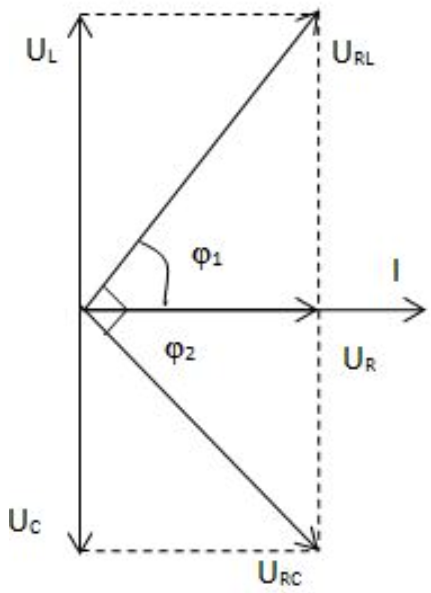
\includegraphics[scale=0.8]{../figs/VN12-2021-PH-TP024-3}
		\end{center}
	
		Ta có:
		$$\tan \varphi_1 \cdot \tan \varphi_2 = 1 \Rightarrow \dfrac{Z_L}{R} \cdot \dfrac{Z_C}{R} = 1 \Rightarrow R^2 = Z_L \cdot Z_C.$$
	}
	
	\item \mkstar{2}
	
	\cauhoi{
		Đoạn mạch $RLC$ mắc nối tiếp, cuộn dây thuần cảm. Gọi $U_R$, $U_L$, $U_C$ lần lượt là điện áp hiệu dụng ở hai đầu điện trở, cuộn cảm thuần và tụ điện. Biết $U_L = 2 U_R = 2 U_C$. Kết luận nào sau đây là đúng?
		
		\begin{mcq}(2)
			\item $u$ sớm pha hơn $i$ một góc $\dfrac{\pi}{4}\ \text{rad}$.
			\item $u$ chậm pha hơn $i$ một góc $\dfrac{\pi}{4}\ \text{rad}$.
			\item $u$ sớm pha hơn $i$ một góc $\dfrac{3\pi}{4}\ \text{rad}$.
			\item $u$ chậm pha hơn $i$ một góc $\dfrac{3\pi}{4}\ \text{rad}$.
		\end{mcq}
	}
	\loigiai{
		\textbf{Đáp án A.}
		
		Áp dụng $\tan \varphi = \dfrac{U_L - U_C}{U_R} = \dfrac{2U_R - U_R}{U_R} = 1$, suy ra $u$ sớm pha hơn $i$ một góc $\dfrac{\pi}{4}\ \text{rad}$.
	}
	
	\item \mkstar{2}
	
	\cauhoi{
		Cho đoạn mạch điện $RLC$ nối tiếp. Đặt vào hai đầu mạch một điện áp xoay chiều ổn định $u$ thì điện áp giữa hai đầu các phần tử là $U_R = \sqrt{3} U_C$, $U_L = 2 U_C$. Độ lệch pha giữa điện áp hai đầu đoạn mạch và cường độ dòng điện là
		
		\begin{mcq}(4)
			\item $\dfrac{\pi}{6}\ \text{rad}$.
			\item $-\dfrac{\pi}{6}\ \text{rad}$.
			\item $\dfrac{\pi}{3}\ \text{rad}$.
			\item $-\dfrac{\pi}{3}\ \text{rad}$.
		\end{mcq}
	}
	\loigiai{
		\textbf{Đáp án A.}
		
		Áp dụng $\tan \varphi = \dfrac{U_L - U_C}{U_R} = \dfrac{2U_C - U_C}{\sqrt{3} U_C} = \dfrac{1}{\sqrt{3}}$, suy ra $u$ sớm pha hơn $i$ một góc $\dfrac{\pi}{6}\ \text{rad}$.
	}
	
	\item \mkstar{2}
	
	\cauhoi{
		Cho đoạn mạch $RLC$ mắc nối tiếp ($L$ là cuộn dây thuần cảm). Điện áp hiệu dụng giữa hai bản tụ điện là $U_C = \SI{160}{V}$, hai đầu đoạn mạch là $U=\SI{160}{V}$. Điện áp trên tụ điện lệch pha so với điện áp hai đầu đoạn mạch là $\dfrac{\pi}{3}\ \text{rad}$. Điện áp hiệu dụng giữa hai đầu cuộn cảm là
		
		\begin{mcq}(4)
			\item $\SI{80}{V}$.
			\item $\xsi{40\sqrt{3}}{V}$.
			\item $\SI{120}{V}$.
			\item $\SI{90}{V}$.
		\end{mcq}
	}
	\loigiai{
		\textbf{Đáp án A.}
		
		Dựa vào giản đồ vectơ:
		\begin{center}
			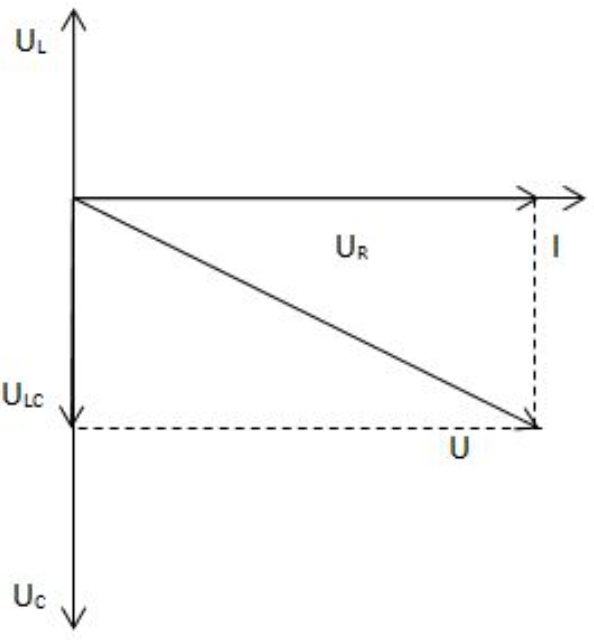
\includegraphics[scale=0.8]{../figs/VN12-2021-PH-TP024-4}
		\end{center}
	
		Ta có:
		$$U_{LC} = U \cos \dfrac{\pi}{3} = \dfrac{U}{2} = \SI{80}{V}.$$
		
		Điện áp hiệu dụng giữa hai đầu cuộn cảm:
		$$U_L = U_C - U_{LC} = \SI{80}{V}.$$
	}
	
	\item \mkstar{2}
	
	\cauhoi{
		Một đoạn mạch gồm cuộn dây có điện trở trong $R=\xsi{100\sqrt{3}}{\Omega}$, độ tự cảm $L$ mắc nối tiếp với tụ điện có điện dung $C=\xsi{\dfrac{5\cdot 10^{-5}}{\pi}}{F}$. Đặt vào hai đầu đoạn mạch một hiệu điện thế xoay chiều $u=U_0 \cos \left(100 \pi t - \dfrac{\pi}{4}\right)\ \text V$ thì cường độ dòng điện tức thời trong mạch là $i=\sqrt{2} \cos \left(100 \pi t - \dfrac{\pi}{12}\right)\ \text A$. Độ tự cảm của cuộn dây là
		
		\begin{mcq}(4)
			\item $\xsi{\dfrac{0,4}{\pi}}{H}$.
			\item $\xsi{\dfrac{0,5}{\pi}}{H}$.
			\item $\xsi{\dfrac{0,6}{\pi}}{H}$.
			\item $\xsi{\dfrac{1}{\pi}}{H}$.
		\end{mcq}
	}
	\loigiai{
		\textbf{Đáp án D.}
		
		Dung kháng của tụ điện:
		$$Z_C = \dfrac{1}{\omega C} = \SI{200}{\Omega}.$$
		
		Ta có $\varphi = \varphi_u - \varphi_i = \xsi{-\dfrac{\pi}{6}}{rad}$, suy ra:
		$$\tan \varphi = \dfrac{Z_L - Z_C}{R} = \tan (-\dfrac{\pi}{6}) = - \dfrac{\sqrt{3}}{3} \Rightarrow Z_L = \SI{100}{\Omega}.$$
		
		Vậy $L=\dfrac{Z_L}{\omega} = \xsi{\dfrac{1}{\pi}}{H}$.
	}
	
	\item \mkstar{3}
	
	\cauhoi{
		Một đoạn mạch gồm điện trở $R=\SI{100}{\Omega}$ mắc nối tiếp với tụ điện có điện dung $C=\dfrac{10^{-4}}{\pi}\ \text F$. Đặt vào hai đầu mạch một điện áp xoay chiều $u=200 \cos (100\pi t)\ \text V$. Cường độ dòng điện hiệu dụng qua mạch là
		
		\begin{mcq}(4)
			\item $\xsi{1,2\sqrt{2}}{A}$.
			\item $\SI{1}{A}$.
			\item $\SI{2}{A}$.
			\item $\xsi{\sqrt{2}}{A}$.
		\end{mcq}
	}
	\loigiai{
		\textbf{Đáp án B.}
		
		Trở kháng toàn mạch:
		$$Z = \sqrt{R^2 + Z_C^2} = \SI{100}{\Omega}.$$
		
		Cường độ dòng điện hiệu dụng toàn mạch:
		$$I=\dfrac{U}{Z} = \SI{1}{A}.$$
	}
	
	\item \mkstar{3}
	
	\cauhoi{
		Một mạch điện gồm điện trở thuần $R=\SI{100}{\Omega}$ mắc nối tiếp với cuộn cảm thuần có độ tự cảm $L=\dfrac{1}{\pi}\ \text H$. Đặt vào hai đầu đoạn mạch một điện áp xoay chiều $u=200 \cos(100\pi t)\ \text V$. Công suất tiêu thụ của mạch điện là
		
		\begin{mcq}(4)
			\item $\xsi{200\sqrt{2}}{W}$.
			\item $\SI{200}{W}$.
			\item $\SI{100}{W}$.
			\item $\SI{50}{W}$.
		\end{mcq}
	}
	\loigiai{
		\textbf{Đáp án C.}
		
		Trở kháng toàn mạch:
		$$Z=\sqrt{R^2 + Z_L^2} = \xsi{100\sqrt{2}}{\Omega}.$$
		
		Cường độ dòng điện hiệu dụng toàn mạch:
		$$I=\dfrac{U}{Z} = \SI{1}{A}.$$
		
		Công suất tiêu thụ:
		$$\calP = I^2 R = \SI{100}{W}.$$
	}
	
	\item \mkstar{3}
	
	\cauhoi{
		Cho một đoạn mạch điện xoay chiều gồm các đoạn mắc nối tiếp nhau: đoạn AM chứa tụ điện, đoạn MN chứa cuộn cảm thuần, đoạn NB chứa điện trở thuần. Biết $U_\text{AM} = \SI{40}{V}$, $U_\text{MB} = \xsi{20\sqrt 2}{V}$, $U_\text{AB} = \xsi{20\sqrt{2}}{V}$. Hệ số công suất của mạch bằng
		
		\begin{mcq}(4)
			\item $\dfrac{\sqrt{2}}{2}$.
			\item $\dfrac{1}{2}$.
			\item $\sqrt{2}$.
			\item $\dfrac{1}{4}$.
		\end{mcq}
	}
	\loigiai{
		\textbf{Đáp án A.}
		
		Ta có $U_C = U_\text{AM}$, $U_L = U_\text{MN}$, $U_R = U_\text{NB}$, $U_{RL} = U_\text{MB}$.
		
		Mặt khác, ta có $U_{RL}^2 = U_R^2 + U_L^2$ và $U_\text{AB}^2 = U_R^2 + U_L^2 + U_C^2 - 2 U_L U_C$.
		
		Suy ra $U_C^2 = 2 U_L U_C \Rightarrow U_L =\dfrac{U_C}{2} = \SI{20}{V}$ và $U_R=\SI{20}{V}$.
		
		Vậy hệ số công suất là
		$$\cos \varphi = \dfrac{U_R}{U_\text{AB}} = \dfrac{\sqrt{2}}{2}.$$
	}
	
	\item \mkstar{3}
	
	\cauhoi{
		Cho đoạn mạch xoay chiều $RLC$ nối tiếp. Biết điện áp đặt vào hai đầu đoạn mạch là $u=100 \cos 100 \pi t\ \text V$, điện áp hiệu dụng giữa hai đầu cuộn cảm thuần là $U_L = \SI{50}{V}$, công suất tiêu thụ trên đoạn mạch $\calP = \SI{50}{W}$ và dòng điện sớm pha $\dfrac{\pi}{4}\ \text{rad}$ so với điện áp. Điện trở $R$ và dung kháng $Z_C$ có giá trị là
		
		\begin{mcq}(2)
			\item $R=\SI{100}{\Omega}$, $Z_C = \SI{50}{\Omega}$.
			\item $R=\SI{50}{\Omega}$, $Z_C = \SI{50}{\Omega}$.
			\item $R=\SI{50}{\Omega}$, $Z_C = \SI{100}{\Omega}$.
			\item $R=\SI{100}{\Omega}$, $Z_C = \SI{100}{\Omega}$.
		\end{mcq}
	}
	\loigiai{
		\textbf{Đáp án C.}
		
		Ta có $\tan \varphi = \dfrac{U_L - U_C}{U_R} = \tan \dfrac{\pi}{4} = 1$. Suy ra $U_L - U_C = U_R$.
		
		Với $\calP = UI \cos \varphi = \SI{50}{W}$, trong đó $U=\sqrt{U_R^2 + (U_L - U_C)^2} = \sqrt{2U_R^2}$ và $I=\dfrac{U_R}{R}$. Tính được $R=\SI{50}{\Omega}$ và $Z_C = \SI{100}{\Omega}$.
	}
	
	\item \mkstar{3}
	
	\cauhoi{
		Cho đoạn mạch điện xoay chiều gồm điện trở thuần $R$ và tụ điện có điện dung $C=\dfrac{10^{-4}}{3\pi}\ \text F$ mắc vào mạch điện xoay chiều có giá trị điện áp hiệu dụng $\SI{150}{V}$, tần số $\SI{50}{Hz}$ và cường độ dòng điện trong mạch có giá trị hiệu dụng là $\dfrac{\sqrt{5}}{5}\ \text{A}$. Điện trở thuần $R$ có giá trị bằng
		
		\begin{mcq}(4)
			\item $\SI{50}{\Omega}$.
			\item $\SI{150}{\Omega}$.
			\item $\SI{200}{\Omega}$.
			\item $\SI{100}{\Omega}$.
		\end{mcq}
	}
	\loigiai{
		\textbf{Đáp án B.}
		
		Dung kháng của tụ điện:
		$$Z_C = \dfrac{1}{\omega C} = \SI{300}{\Omega}.$$
		
		Trở káng của toàn mạch:
		$$Z=\sqrt{R^2  + Z_C^2} = \dfrac{U}{I} = \xsi{150\sqrt{5}}{\Omega}.$$
		
		Suy ra $R=\SI{150}{\Omega}$.
	}
	
	\item \mkstar{3}
	
	\cauhoi{
		Cho mạch điện $RLC$ như hình vẽ.
		\begin{center}
			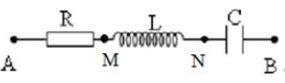
\includegraphics[scale=1]{../figs/VN12-2021-PH-TP024-1.png}
		\end{center}
		
		Cho điện áp hai đầu mạch là $u_\text{AB} = 200 \sqrt{2} \cos 100 \pi t\ \text{V}$ và điện trở $R=\xsi{100\sqrt{3}}{\Omega}$. Điện áp hai đầu đoạn mạch MN nhanh pha hơn hiệu điện thế hai đầu mạch AB một góc $\xsi{\dfrac{2\pi}{3}}{rad}$. Cường độ dòng điện $i$ qua mạch có biểu thức:
		\begin{mcq}(2)
			\item $i=\sqrt{2} \cos \left(100 \pi t + \dfrac{\pi}{6}\right)\ \text A$.
			\item $i=\sqrt{2} \cos \left(100 \pi t + \dfrac{\pi}{3}\right)\ \text A$.
			\item $i=\sqrt{2} \cos \left(100 \pi t - \dfrac{\pi}{3}\right)\ \text A$.
			\item $i=\sqrt{2} \cos \left(100 \pi t - \dfrac{\pi}{6}\right)\ \text A$.
		\end{mcq}
	}
	\loigiai{
		\textbf{Đáp án A.}
		
		Giả sử cuộn dây là thuần cảm, ta có giản đồ vectơ:
		\begin{center}
			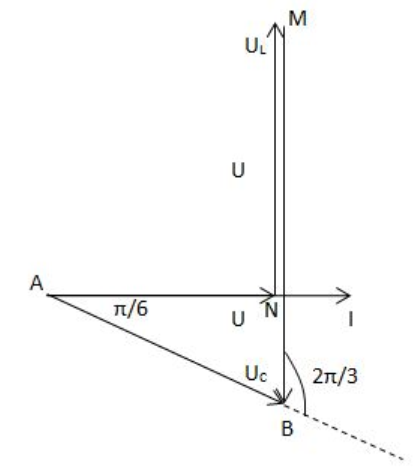
\includegraphics[scale=0.8]{../figs/VN12-2021-PH-TP024-5}
		\end{center}
	
		Xét tam giác vuông NAB, có: $\text{AB} = \dfrac{\text{AN}}{\cos \dfrac{\pi}{6}} = \dfrac{2}{\sqrt{3}} \text{AN}$, hay $Z=\dfrac{2}{\sqrt{3}} R = \SI{200}{\Omega}$.
		
		Cường độ dòng điện cực đại:
		$$I_0 = \dfrac{U_0}{Z} = \xsi{\sqrt{2}}{A}.$$
		
		Vì $i$ sớm pha hơn $u$ một góc $\dfrac{\pi}{6}\ \text{rad}$, nên biểu thức của $i$ là
		$$i=\sqrt{2} \cos \left(100 \pi t + \dfrac{\pi}{6}\right)\ \text{A}.$$
	}
	
	\item \mkstar{3}
	
	\cauhoi{
		Cho mạch điện như hình vẽ.
		\begin{center}
			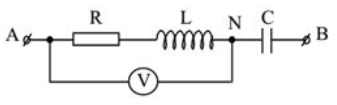
\includegraphics[scale=1]{../figs/VN12-2021-PH-TP024-2.png}
		\end{center}
	
	Với $U_\text{AB} = \SI{300}{V}$, $U_\text{NB} = \SI{140}{V}$, dòng điện $i$ trễ pha so với $u_\text{AB}$ một góc $\varphi$ (với $\cos \varphi = \SI{0.8}{}$), cuộn dây thuần cảm. Vôn kế V chỉ giá trị
		\begin{mcq}(4)
			\item $\SI{100}{V}$.
			\item $\SI{200}{V}$.
			\item $\SI{300}{V}$.
			\item $\SI{400}{V}$.
		\end{mcq}
	}
	\loigiai{
		\textbf{Đáp án D.}
		
		Ta có giản đồ vectơ:
		\begin{center}
			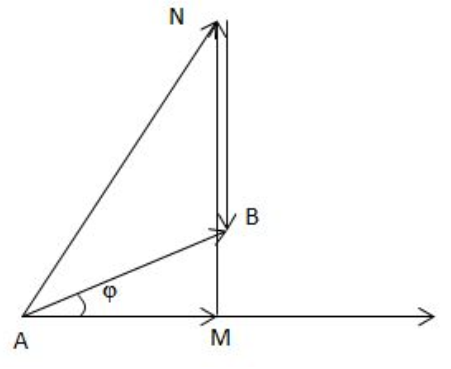
\includegraphics[scale=0.8]{../figs/VN12-2021-PH-TP024-6}
		\end{center}
	
	Trong tam giác vuông MAB có $\widehat{\text{MBA}} = \varphi = 90^\circ$, suy ra $\cos \varphi = \sin \widehat{\text{MBA}} = \SI{0.8}{}$.
	
	Mà lại có $\widehat{\text{MBA}} + \widehat{\text{ABN}} = 180^\circ$, suy ra: $\sin \widehat{\text{ABN}} = \sin \widehat{\text{MBA}} = \SI{0.8}{}$.
	
	Do đó $\cos \widehat{\text{ABN}} = \pm \sqrt{1 - \sin^2 \widehat{\text{ABN}}} = \pm \SI{0.6}{}$.
	
	Vì $\widehat{\text{ABN}}$ là góc tù nên $\cos \widehat{\text{ABN}} = \SI{-0.6}{}$.
	
	Trong tam giác ABN có: $\text{AN}^2 = \text{AB}^2 + \text{BN}^2 - 2 \cdot \text{AB} \cdot \text{BN} \cos \widehat{\text{ABN}}$, hay
	$$U_\text{AN}^2 = U_\text{AB}^2 + U_\text{NB}^2 - 2 U_\text{AB} U_\text{NB} \cos \widehat{\text{ABN}}.$$
	
	Thay số, ta được: $U_\text{AN} = \SI{400}{V}$.
	}
	
	\item \mkstar{3}
	
	\cauhoi{
		Mạch điện xoay chiều gồm điện trở thuần $R=\SI{30}{\Omega}$ mắc nối tiếp với cuộn dây. Đặt vào hai đầu mạch một điện áp xoay chiều $u=U\sqrt{2} \cos (100 \pi t)\ \text V$. Điện áp hiệu dụng ở hai đầu cuộn dây là $U_\text{d} = \SI{60}{V}$. Dòng điện trong mạch lệch pha $\dfrac{\pi}{6}\ \text{rad}$ so với $u$ và lệch pha $\dfrac{\pi}{3}\ \text{rad}$ so với $u_\text{d}$. Điện áp hiệu dụng ở hai đầu mạch có giá trị là
		
		\begin{mcq}(4)
			\item $U=\xsi{60\sqrt{2}}{V}$.
			\item $U=\SI{120}{V}$.
			\item $U=\SI{90}{V}$.
			\item $U=\xsi{60\sqrt{3}}{V}$.
		\end{mcq}
	}
	\loigiai{
		\textbf{Đáp án D.}
		
		Do dòng điện trong mạch lệch pha $\dfrac{\pi}{3}\ \text{rad}$ so với $u_\text{d}$ nên cuộn dây không thuần cảm. Giản đồ vectơ:
		\begin{center}
			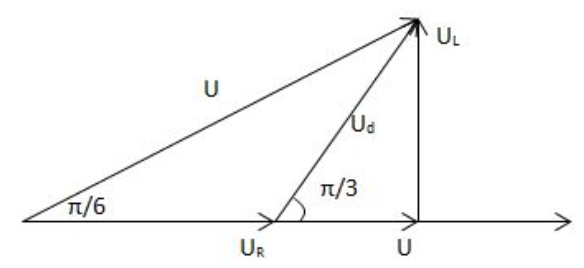
\includegraphics[scale=0.8]{../figs/VN12-2021-PH-TP024-7}
		\end{center}
	
	Ta có:
	$$U_\text{d} = U_R = \SI{60}{V}.$$
	$$U^2 = U_R^2 + U_\text{d}^2 - 2 U_R U_\text{d} \cos \dfrac{2\pi}{3}$$
	
	Thay số, ta được: $U=\xsi{60\sqrt 3}{V}$.
	}
	
	\item \mkstar{3}
	
	\cauhoi{
		Cho đoạn mạch điện xoay chiều gồm điện trở $R$, cuộn cảm thuần có độ tự cảm $L=\dfrac{0,2}{\pi}\ \text H$ và tụ điện $C=\dfrac{10^{-4}}{\pi}$ mắc nối tiếp. Đặt vào hai đầu đoạn mạch một điện áp xoay chiều có giá trị hiệu dụng $U=\SI{200}{V}$, tần số $\SI{50}{Hz}$. Để công suất tiêu thụ trên đoạn mạch là $\calP = \SI{240}{W}$ thì giá trị của điện trở là
		
		\begin{mcq}(2)
			\item $\SI{60}{\Omega}$ hoặc $\SI{160}{\Omega}$.
			\item $\SI{60}{\Omega}$ hoặc $\SI{106.7}{\Omega}$.
			\item $\SI{60}{\Omega}$ hoặc $\SI{30}{\Omega}$.
			\item $\SI{60}{\Omega}$ hoặc $\SI{180}{\Omega}$.
		\end{mcq}
	}
	\loigiai{
		\textbf{Đáp án B.}
		
		Công suất:
		$$\calP = I^2 R = \dfrac{U^2}{R^2 + (Z_L - Z_C)^2} R \Rightarrow \calP R^2 - U^2 R + \calP(Z_L - Z_C)^2 = 0$$
		$$\Rightarrow 240R^2 - 40000R + 1536000 = 0$$
		
		Vậy $R=\SI{60}{\Omega}$ hoặc $R=\SI{106.67}{\Omega}$.
		
	}
	
	\item \mkstar{3}
	
	\cauhoi{
		Cho đoạn mạch xoay chiều $RLC$ nối tiếp. Đặt vào hai đầu đoạn mạch điện áp $u=100\sqrt{2} \cos 100 \pi t\ \text V$. Biết công suất tiêu thụ trên đoạn mạch là $\SI{100}{W}$, dòng điện chạy trong mạch nhanh hơn điện áp một góc $\dfrac{\pi}{4}$ và điện áp hiệu dụng giữa hai đầu cuộn cảm thuần là $\xsi{50\sqrt{2}}{V}$. Điện dung $C$ của tụ điện có giá trị bằng
		
		\begin{mcq}(4)
			\item $\dfrac{4\cdot10^{-4}}{\pi}\ \text F$.
			\item $\dfrac{2\cdot 10^{-4}}{\pi}\ \text F$.
			\item $\dfrac{10^{-4}}{\pi}\ \text F$.
			\item $\SI{26.38}{F}$.
		\end{mcq}
	}
	\loigiai{
		\textbf{Đáp án C.}
		
		Ta có $\tan \varphi = \dfrac{U_L - U_C}{R} =\tan \dfrac{\pi}{4} = 1$, suy ra $U_L - U_C = U_R$.
		
		Vì $u=\sqrt{U_R^2 + (U_L - U_C)^2} = \sqrt{2 (U_L - U_C)^2}$, suy ra $U_L - U_C = 50\sqrt{2}$.
		
		Tính được: $U_C = \xsi{100\sqrt{2}}{V}$ và $U_R = \xsi{50\sqrt 2}{V}$.
		
		Mà $\calP = U_R I$, suy ra:
		$$I = \dfrac{\calP}{U_R} = \xsi{\sqrt{2}}{A}.$$
		
		Vậy $Z_C = \dfrac{U_C}{I} = \SI{100}{\Omega}$ hay $C=\dfrac{1}{\omega C} = \dfrac{10^{-4}}{\pi}\ \text{F}$.
	}
	
	\item \mkstar{3}
	
	\cauhoi{
		Một đoạn mạch xoay chiều gồm hai trong ba phần tử mắc nối tiếp: điện trở thuần $R$, tụ điện có dung kháng $Z_C$, cuộn cảm có cảm kháng $Z_L$. Biết điện áp xoay chiều giữa hai đầu đoạn mạch là $u=120 \sqrt{2} \cos (100\pi t)\ \text V$. Cường độ dòng điện qua mạch có biểu thức $i=1,2 \cos \left(100 \pi t - \dfrac{\pi}{4}\right)\ \text A$. Thông số của hai phần tử đó là
		
		\begin{mcq}(2)
			\item $R=Z_L = \SI{100}{\Omega}$.
			\item $R=Z_C = \SI{100}{\Omega}$.
			\item $Z_L = Z_C = \xsi{25\sqrt{2}}{\Omega}$.
			\item $R=Z_L = \xsi{25\sqrt{2}}{\Omega}$.
		\end{mcq}
	}
	\loigiai{
		\textbf{Đáp án A.}
		
		Vì $u$ sớm pha hơn $i$ nên đoạn mạch gồm hai phần tử nối tiếp: $R$ và $L$. Khi đó:
		$$Z=\sqrt{R^2 + Z_L^2} = \dfrac{U}{I} = \xsi{100\sqrt 2}{\Omega}.$$
		
		Mà $\tan \varphi = \dfrac{Z_L}{R} = \tan \dfrac{\pi}{4} = 1$, nên $R=Z_L = \SI{100}{\Omega}$.
	}
	
	\item \mkstar{3}
	
	\cauhoi{
		Cho đoạn mạch xoay chiều $RLC$ nối tiếp, trong đó $L$ thay đổi được. Điện áp đặt vào hai đầu đoạn mạch có biểu thức $u=200 \sqrt{2} \cos 100 \pi t \ \text V$. Biết khi $L=L_1 = \dfrac{3\sqrt{3}}{\pi}\ \text H$ và khi $L=L_2 = \dfrac{\sqrt{3}}{\pi}\ \text{H}$ thì cường độ dòng điện hiệu dụng chạy trong đoạn mạch đều bằng nhau, nhưng giá trị tức thời lệch pha nhau một góc là $\dfrac{2\pi}{3}\ \text{rad}$. Điện trở $R$ có giá trị bằng
		
		\begin{mcq}(4)
			\item $\xsi{200\sqrt{3}}{\Omega}$.
			\item $\SI{200}{\Omega}$.
			\item $\xsi{100\sqrt{3}}{\Omega}$.
			\item $\SI{100}{\Omega}$.
		\end{mcq}
	}
	\loigiai{
		\textbf{Đáp án D.}
		
		Vì khi $L = L_1$ hoặc $L=L_2$ thì $i_1 = i_2 = i$ nên ta có $Z_1 = Z_2$. Khi đó:
		$$Z_C = \dfrac{Z_{L1} + Z_{L2}}{2} = \xsi{200\sqrt{3}}{\Omega}.$$
		
		Mặt khác, ta lại có:
		$$\tan (\varphi_1 + \varphi_2) = \dfrac{\tan \varphi_1 + \tan \varphi_2}{1 - \tan \varphi_1 \cdot \tan \varphi_2} = \tan \dfrac{2\pi}{3} = -\sqrt{3}.$$
		
		Thay $\tan \varphi_1 = \dfrac{Z_{L1} - Z_C}{R}$ và $\tan \varphi_2 = \dfrac{Z_C - Z_{L2}}{R}$, ta được $R=\SI{100}{\Omega}$.
	}
	
	\item \mkstar{3}
	
	\cauhoi{
		Cho một đoạn mạch điện xoay chiều gồm các đoạn mắc nối tiếp nhau: đoạn AM chứa tụ điện, đoạn MN chứa điện trở thuần, đoạn NB chứa cuộn cảm thuần. Biết $U_\text{AN} = \SI{200}{V}$, $U_\text{MB} = \SI{150}{V}$, điện áp tức thời $u_\text{AN}$ vuông pha với $u_\text{MB}$, cường độ dòng điện trong mạch có giá trị hiệu dụng $\SI{2}{A}$, tần số $\SI{50}{Hz}$. Độ tự cảm có giá trị bằng
		
		\begin{mcq}(4)
			\item $\dfrac{0,45}{\pi}\ \text{H}$.
			\item $\dfrac{1,45}{\pi}\ \text H$.
			\item $\SI{0,45}{H}$.
			\item $\SI{0.25}{H}$.
		\end{mcq}
	}
	\loigiai{
		\textbf{Đáp án A.}
		
		Trở kháng của đoạn AN là $Z_\text{AN} = \sqrt{R^2 + Z_C^2} = \dfrac{U_\text{AN}}{I} = \SI{100}{\Omega}$, suy ra:
		$$R^2 + Z_C^2 = 100^2.$$
		
		Trở kháng của đoạn MB là $Z_{MB} = \sqrt{R^2 + Z_L^2} = \dfrac{U_\text{MB}}{I} = \SI{75}{\Omega}$, suy ra:
		$$R^2 + Z_L^2 = 75^2.$$
		
		Mà $u_\text{AN}$ vuông pha với $u_\text{MB}$ nên:
		$$\tan \varphi_\text{AN} \cdot \tan \varphi_\text{MB} = 1 \Rightarrow \dfrac{Z_C}{R} \cdot \dfrac{Z_L}{R} = 1 \Rightarrow Z_L Z_C = R^2.$$
		
		Giải hệ 3 phương trình trên, tìm được $Z_L = \SI{45}{\Omega}$ hay $L=\dfrac{0,45}{\pi}\ \text{H}$.
	}
	
	\item \mkstar{3}
	
	\cauhoi{
		Cho đoạn mạch xoay chiều gồm các phần tử $R$, $L$, $C$ mắc nối tiếp, trong đó $R$ thay đổi được, $Z_L = \SI{15}{\Omega}$, $Z_C = \SI{4}{\Omega}$, điện áp đặt vào hai đầu đoạn mạch là $u=12\sqrt{2} \cos 100 \pi t \ \text V$. Công suất tiêu thụ của đoạn mạch đạt cực đại khi $R$ bằng
		
		\begin{mcq}(4)
			\item $\SI{11}{\Omega}$.
			\item $\SI{6}{\Omega}$.
			\item $\SI{2}{\Omega}$.
			\item $\SI{14}{\Omega}$.
		\end{mcq}
	}
	\loigiai{
		\textbf{Đáp án A.}
		
		$R$ thay đổi để $\calP_\text{max}$ khi $R=|Z_L - Z_C|$, khi đó $R=\SI{11}{\Omega}$.
	}
	
	\item \mkstar{3}
	
	\cauhoi{
		Cho mạch điện gồm $R$, $L$, $C$ mắc nối tiếp. Biết điện trở $R$ không thay đổi, hệ số tự cảm $L=\dfrac{0,5}{\pi}\ \text H$, tụ điện có điện dung $C$ thay đổi được. Đặt vào hai đầu đoạn mạch một điện áp ổn định có biểu thức $u=200 \sqrt{2} \cos (100\pi t)\ \text V$. Giá trị của $C$ để công suất tiêu thụ trong mạch đạt cực đại là
		
		\begin{mcq}(4)
			\item $\dfrac{0,1}{\pi}\ \text F$.
			\item $\dfrac{10^{-2}}{\pi}\ \text F$.
			\item $\dfrac{10^{-3}}{\pi}\ \text F$.
			\item $\dfrac{2\cdot 10^{-4}}{\pi}\ \text F$.
		\end{mcq}
	}
	\loigiai{
		\textbf{Đáp án D.}
		
		Thay đổi $C$ để $\calP_\text{max}$ thì trong mạch xảy ra cộng hưởng, khi đó:
		$$Z_L = Z_C \Rightarrow C = \dfrac{1}{\omega^2 L} = \dfrac{2 \cdot 10^{-4}}{\pi}\ \text{F}.$$
	}
	
	\item \mkstar{4}
	
	\cauhoi{
		Đặt điện áp xoay chiều có giá trị hiệu dụng không đổi $\SI{150}{V}$ vào đoạn mạch AMB gồm AM chỉ chứa điện trở $R$, đoạn MB chứa tụ điện có điện dung C mắc nối tiếp với một cuộn cảm thuần có độ tự cảm $L$ thay đổi được. Biết sau khi thay đổi độ tự cảm $L$ thì điện áp hiệu dụng hai đầu đoạn mạch MB tăng $2\sqrt{2}$ lần và dòng điện trong mạch trước sau thay đổi pha một góc $\dfrac{\pi}{2}\ \text{rad}$. Tìm điện áp hiêu jdụng hai đầu đoạn mạch AM khi chưa thay đổi $L$.
		
		\begin{mcq}(4)
			\item $\SI{100}{V}$.
			\item $\xsi{100\sqrt{2}}{V}$.
			\item $\xsi{100\sqrt{3}}{V}$.
			\item $\SI{120}{V}$.
		\end{mcq}
	}
	\loigiai{
		\textbf{Đáp án B.}
		
		Gọi $\varphi_1$, $\varphi_2$ lần lượt là độ lệch pha giữa $u$ và $i$ trước và sau khi thay đổi $L$.
		$$\tan \varphi_1 = \dfrac{U_{L1} - U_{C1}}{U_{R1}}$$
		$$\tan \varphi_2 = \dfrac{U_{L2} - U_{C2}}{U_{R2}}$$
		
		Ta có $i_1$ và $i_2$ vuông pha với nhau nên:
		$$\varphi_1 + \varphi_2 = \dfrac{\pi}{2} \Rightarrow \tan \varphi_1 \cdot \tan \varphi_2 = -1.$$
		
		Thay các đại lượng vào, ta được:
		$$(U_{L1} - U_{C1})^2 \cdot (U_{L2} - U_{C2})^2 = U_{R1}^2 U_{R2}^2 \Rightarrow 8 U_\text{MB1}^2 = U_{R1}^2 U_{R2}^2.$$
		
		Mặt khác:
		$$U_{R1}^2 + U_\text{MB1}^2 = U_{R2}^2 + U_\text{MB2}^2 = U^2 \Rightarrow U_{R2}^2 = U_{R1}^2 - 7 U_\text{MB1}^2.$$
		
		Suy ra $8 U_\text{MB1}^2 = U_{R1}^2 \cdot (U_{R1}^2 - 7 U_\text{MB1}^2)$, hay:
		$$U_{R1}^2 = 8 U_\text{MB1}^2.$$
		
		Ngoài ra thì $U_{R1}^2 + U_\text{MB1}^2 = U^2$. Tính được:
		$$U_{R1} = 2 \cdot \dfrac{\sqrt{2}}{3} \cdot U = \xsi{100\sqrt{2}}{V}.$$
	}
	
	\item \mkstar{4}
	
	\cauhoi{
		Một đoạn mạch AB gồm 3 phần tử $R$, $L$, $C$ mắc nối tiếp (cuộn dây thuần cảm có độ tự cảm $L$). Đặt điện áp xoay chiều $u=U\sqrt{2} \cos 2\pi f t\ \text V$ ($U$ không đổi, $f$ thay đổi được) vào hai đầu đoạn mạch AB. Khi tần số là $f=f_0$ thì dòng điện sớm pha $\dfrac{\pi}{4}\ \text{rad}$ so với điện áp hai đầu mạch AB và lúc đó cảm kháng bằng với giá trị của $R$. Khi tần số là $f=f_1 = 2f_0$ thì độ lệch pha giữa điện áp hai đầu mạch AB so với cường độ dòng điện là
		
		\begin{mcq}(4)
			\item $\dfrac{\pi}{3}\ \text{rad}$.
			\item $\dfrac{\pi}{4}\ \text{rad}$.
			\item $\dfrac{\pi}{6}\ \text{rad}$.
			\item $-\dfrac{\pi}{4}\ \text{rad}$.
		\end{mcq}
	}
	\loigiai{
		\textbf{Đáp án B.}
		
		Sử dụng phương pháp chuẩn hóa số liệu, cho $Z_L = R = 1$ khi $f=f_0$.
		
		Khi $f=f_0$, dòng điện sớm pha $\dfrac{\pi}{4}\ \text{rad}$ so với điện áp hai đầu đoạn mach:
		$$\tan (-\dfrac{\pi}{4}) = \dfrac{Z_{L0} - Z_{C0}}{R} = -1 \Rightarrow Z_{C0} - Z_{L0} = R = 1 \Rightarrow Z_{C0} = 2.$$
		
		Khi $f=f_1=2f_0$ thì $Z_{L1} = 2 Z_{L0} = 2$ và $Z_{C1} = 1$:
		$$\tan \varphi_1 = \dfrac{Z_{L1} - Z_{C1}}{R} = 1.$$
		
		Vậy $\varphi_1 = \dfrac{\pi}{4}\ \text{rad}$.
	}
	
	\item \mkstar{4}
	
	\cauhoi{
		Đặt điện áp $u=U\sqrt{2} \cos 2\pi f t\ \text{V}$ ($U$ không đổi, $f$ thay đổi được) vào hai đầu đoạn mạch mắc nối tiếp gồm điện trở thuần $R$, cuộn cảm thuần có độ tự cảm $L$ và tụ điện có điện dung $C$. Khi tần số là $f_1$ thì cảm kháng và dung kháng của đoạn mạch có giá trị lần lượt là $\SI{6}{\Omega}$ và $\SI{8}{\Omega}$. Khi tần số là $f_2$ thì hệ số công suất của đoạn mạch bằng 1. Hệ thức liên hệ giữa $f_1$ và $f_2$ là
		
		\begin{mcq}(2)
			\item $f_2 =\dfrac{4}{3} f_1$.
			\item $f_2 = \dfrac{\sqrt{3}}{2} f_1$.
			\item $f_2 = \dfrac{2}{\sqrt{3}} f_1$.
			\item $f_2 = \dfrac{3}{4} f_1$.
		\end{mcq}
	}
	\loigiai{
		\textbf{Đáp án C.}
		
		Giả sử $f_2 = n f_1$, ta có:
		$$Z_{L1} = 6 \Rightarrow Z_{L2} = 6n.$$
		$$Z_{C1} = 8 \Rightarrow Z_{C2} = \dfrac{8}{n}.$$
		
		Theo đề, khi tần số là $f_2$ thì $\cos \varphi = 1$, khi đó có hiện tượng cộng hưởng nên $Z_{L2} = Z_{C2}$, hay $6n = \dfrac{8}{n}$, vậy $n=\dfrac{2}{\sqrt{3}}$.
		
		Vậy $f_2 = \dfrac{2}{\sqrt{3}}f_1$.
	}
	
	\item \mkstar{4}
	
	\cauhoi{
		Đặt vào hai đầu cuộn sơ cấp của một máy biến áp lí tưởng (bỏ qua hao phí) một điện áp xoay chiều có giá trị hiệu dụng không đổi thì điện áp hiệu dụng giữa hai đầu cuộn thứ cấp để hở là $\SI{100}{V}$. Ở cuộn thứ cấp, nếu giảm bớt $n$ vòng dây thì điện áp giữa hai đầu để hở của nó là $U$, nếu tăng thêm $n$ vòng dây thì điện áp đó là $2U$. Nếu tăng thêm $3n$ vòng dây ở cuộn thứ cấp thì điện áp hiệu dụng giữa hai đầu để hở của cuộn này bằng
		
		\begin{mcq}(4)
			\item $\SI{100}{V}$.
			\item $\SI{200}{V}$.
			\item $\SI{220}{V}$.
			\item $\SI{110}{V}$.
		\end{mcq}
	}
	\loigiai{
		\textbf{Đáp án B.}
		
		Tỉ số giữa điện áp và số vòng dây ở hai đầu cuộn sơ cấp và thứ cấp:
		$$\dfrac{100}{U_1} = \dfrac{N_2}{N_1}\ (*).$$
		
		Tỉ số giữa điện áp và số vòng dây ở hai đầu cuộn sơ cấp và thứ cấp:
		$$\dfrac{U}{U_1} = \dfrac{N_2 - n}{N_1}\ (**).$$
		
		Tỉ số giữa điện áp và số vòng dây ở hai đầu cuộn sơ cấp và thứ cấp:
		$$\dfrac{2U}{U_1} = \dfrac{N_2 + n}{N_1}\ (***).$$
		
		Lấy $(**)$ cộng $(***)$ và thay $(*)$ vào, suy ra:
		$$\dfrac{2N_2}{N_1} = \dfrac{3U}{U_1} = \dfrac{200}{U_1} \Rightarrow U = \dfrac{200}{3}\ \text{V}.$$
		
		Lấy $(***)$ trừ $(**)$, suy ra:
		$$\dfrac{U}{U_1} = \dfrac{2n}{N_1} \Rightarrow \dfrac{1}{2} \dfrac{U}{U_1} = \dfrac{n}{N_1}.$$
		
		Nếu tăng thêm $3n$ vòng dây thì:
		$$\dfrac{U_2}{U_1} = \dfrac{N_2 + 3n}{N_1} = \dfrac{N_2}{N_1} + 3 \dfrac{n}{N_1} = \dfrac{100}{U_1} + 3 \cdot\dfrac{1}{2} \cdot \dfrac{\frac{200}{3}}{U_1} = \dfrac{200}{U_1}.$$
		
		Suy ra: $U_2 = \SI{200}{V}$.
	}
	
	\item \mkstar{4}
	
	\cauhoi{
		Một máy phát điện xoay chiều ba pha đang hoạt động ổn định. Suất điện động trong ba cuộn dây của phần ứng có giá trị $e_1$, $e_2$ và $e_3$. Ở thời điểm mà $e_1 = \SI{30}{V}$ thì $|e_2 - e_3| = \SI{30}{V}$. Giá trị cực đại của $e_1$ là
		
		\begin{mcq}(4)
			\item $\SI{40.2}{V}$.
			\item $\SI{51.9}{V}$.
			\item $\SI{34.6}{V}$.
			\item $\SI{45.1}{V}$.
		\end{mcq}
	}
	\loigiai{
		\textbf{Đáp án C.}
		
		Giả sử suất điện động trong khung dây có dạng:
		$$
		\begin{cases}
			e_1 = E_0 \cos \omega t \\
			e_2 = E_0 \cos \left(\omega t + \dfrac{2\pi}{3}\right)\\
			e_3 =E_0 \cos \left(\omega t - \dfrac{2\pi}{3}\right)
		\end{cases}
		$$
		
		Theo đề bài:
		$$|e_2 - e_3| = \SI{30}{V} \Rightarrow e_2 - e_3 = \pm \SI{30}{V} \Rightarrow 2 E_0 \sin \omega t \sin \dfrac{2\pi}{3} = \pm \SI{30}{V}.$$
		
		Ngoài ra, cũng theo đề bài:
		$$e_1 = E_0 \cos \omega t = \SI{30}{V}.$$
		
		Ta có hệ phương trình sau:
		$$
		\begin{cases}
			-2E_0 \sin \omega t \sin \dfrac{2\pi}{3} = \pm \SI{30}{V}\\
			E_0 \cos \omega t = \SI{30}{V}
		\end{cases}
		\Rightarrow
		\begin{cases}
			E_0 \sin \omega t = \pm \xsi{10\sqrt{3}}{V}\\
			E_0 \cos \omega t = \SI{30}{V}
		\end{cases}
	\Rightarrow E_0 = \xsi{20\sqrt{3}}{V}=\SI{34.6}{V}.
		$$
	}
\end{enumerate}
\loigiai{\textbf{Đáp án}
	\begin{center}
		\begin{tabular}{|m{2.8em}|m{2.8em}|m{2.8em}|m{2.8em}|m{2.8em}|m{2.8em}|m{2.8em}|m{2.8em}|m{2.8em}|m{2.8em}|}
			\hline
			1. B & 2. C & 3. D & 4. B & 5. B & 6. D & 7. C & 8. D & 9. A & 10. B \\
			\hline
			11. B & 12. D & 13. B & 14. A & 15. A & 16. D & 17. A & 18. A & 19. A & 20. D\\
			\hline
			21. B & 22. C & 23. A & 24. C & 25. B & 26. A & 27. D & 28. D & 29. B & 30. C\\
			\hline
			31. A & 32. D & 33. A & 34. A & 35. D & 36. B & 37. B & 38. C & 39. B & 40. C\\
			\hline
		\end{tabular}
\end{center}}